\documentclass[xcolor=red]{beamer}
\usecolortheme[named=red]{structure}
%\documentclass[10pt, a4paper]{article}
\usepackage{fontspec}
\usepackage{xeCJK} 
\defaultfontfeatures{Mapping=tex-text} % to support TeX conventions like ``---''
\usepackage{xunicode} % Unicode support for LaTeX character names(accents, European chars, etc)
\usepackage{xltxtra} 				% Extra customizations for XeLaTeX
\usepackage{amsmath, amssymb}
\usepackage{enumerate}
\usepackage{graphicx,subfig,float,wrapfig} % support the \includegraphics command and options
\usepackage[outercaption]{sidecap} %[options]=[outercaption], [innercaption], [leftcaption], [rightcaption]
\usepackage{array, booktabs}
\usepackage{color, xcolor}
\usepackage{longtable}
\usepackage{colortbl}                          				
\usepackage{listings}						% 直接將 latex 碼轉換成顯示文字
\usepackage[parfill]{parskip} 				% 新段落前加一空行，不使用縮排
%\usepackage[left=1.5in,right=1in,top=1in,bottom=1in]{geometry} 
\usepackage{url}
\usepackage{amsmath, bm}
\usepackage{upgreek}
\usepackage{lipsum}
\usepackage{adjustbox}
\usepackage{sidecap}
\usepackage{multirow}
\usepackage{tabularx}
\usepackage{makecell}
%\usepackage[french]{babel}
%\usepackage{titling}
% 使用 setspace 套件
\usepackage{setspace}
\usepackage{subcaption}
\usepackage{slashbox}
\graphicspath{{D:/NTPU/LATEX/hw7/images/}}
%-----------------------------------------------------------------
%  中英文內文字型設定
\setCJKmainfont							% 設定中文內文字型
	[
		BoldFont=Microsoft YaHei	    %定義粗體的字型（Win）
%		BoldFont=蘋果儷中黑	    		%定義粗體的字型（Mac）
	]
	{新細明體}						% 設定中文內文字型(Win)
%	{宋體-繁}							% 設定中文內文字型(Mac)	
\setmainfont{Times New Roman}		% 設定英文內文字型
\setsansfont{Arial}					% 無襯字字型 used with {\sffamily ...}
%\setsansfont[Scale=MatchLowercase,Mapping=tex-text]{Gill Sans}
\setmonofont{Courier New}			% 等寬字型 used with {\ttfamily ...}
%\setmonofont[Scale=MatchLowercase]{Andale Mono}
% 其他字型（隨使用的電腦安裝的字型不同，用註解的方式調整（打開或關閉））
% 英文字型
\newfontfamily{\E}{Calibri}				
\newfontfamily{\A}{Arial}
\newfontfamily{\C}[Scale=0.9]{Arial}
\newfontfamily{\R}{Times New Roman}
\newfontfamily{\TT}[Scale=0.8]{Times New Roman}
% 中文字型
\newCJKfontfamily{\MB}{微軟正黑體}				% 等寬及無襯線字體 Win
\newCJKfontfamily{\SM}[Scale=0.8]{新細明體}	% 縮小版(Win)
\newCJKfontfamily{\K}{標楷體}                	% Windows下的標楷體
\newCJKfontfamily{\BB}{Microsoft YaHei}		% 粗體 Win

% 以下為自行安裝的字型：CwTex 組合
\newCJKfontfamily{\CF}{cwTeX Q Fangsong Medium}	% CwTex 仿宋體
\newCJKfontfamily{\CB}{cwTeX Q Hei Bold}			% CwTex 粗黑體
\newCJKfontfamily{\CK}{cwTeX Q Kai Medium}   	% CwTex 楷體
\newCJKfontfamily{\CM}{cwTeX Q Ming Medium}		% CwTex 明體
\newCJKfontfamily{\CR}{cwTeX Q Yuan Medium}		% CwTex 圓體

%-----------------------------------------------------------------------------------------------------------------------
\XeTeXlinebreaklocale "zh"             		%這兩行一定要加，中文才能自動換行
\XeTeXlinebreakskip = 0pt plus 1pt     		%這兩行一定要加，中文才能自動換行
%-----------------------------------------------------------------------------------------------------------------------
\newcommand{\cw}{\texttt{cw}\kern-.6pt\TeX}	% 這是 cwTex 的 logo 文字
\newcommand{\imgdir}{../images/}				% 設定圖檔的目錄位置
\renewcommand{\tablename}{表}	% 改變表格標號文字為中文的「表」（預設為 Table）
\renewcommand{\figurename}{圖}% 改變圖片標號文字為中文的「圖」（預設為 Figure）

% 設定顏色 see color Table: http://latexcolor.com
\definecolor{slight}{gray}{0.9}				
\definecolor{airforceblue}{rgb}{0.36, 0.54, 0.66} 
\definecolor{arylideyellow}{rgb}{0.91, 0.84, 0.42}
\definecolor{babyblue}{rgb}{0.54, 0.81, 0.94}
\definecolor{cadmiumred}{rgb}{0.89, 0.0, 0.13}
\definecolor{coolblack}{rgb}{0.0, 0.18, 0.39}
\definecolor{beaublue}{rgb}{0.74, 0.83, 0.9}
\definecolor{beige}{rgb}{0.96, 0.96, 0.86}
\definecolor{bisque}{rgb}{1.0, 0.89, 0.77}
\definecolor{gray(x11gray)}{rgb}{0.75, 0.75, 0.75}
\definecolor{limegreen}{rgb}{0.2, 0.8, 0.2}
\definecolor{splashedwhite}{rgb}{1.0, 0.99, 1.0}
\definecolor{azure(web)(azuremist)}{rgb}{0.94, 1.0, 1.0}
\definecolor{cadmiumorange}{rgb}{0.93, 0.53, 0.18}
\definecolor{alizarin}{rgb}{0.82, 0.1, 0.26}
\definecolor{cadmiumred}{rgb}{0.89, 0.0, 0.13}
\definecolor{candypink}{rgb}{0.89, 0.44, 0.48}
\definecolor{cream}{rgb}{1.0, 0.99, 0.82}
\definecolor{desertsand}{rgb}{0.93, 0.79, 0.69}
\definecolor{mint}{rgb}{0.24, 0.71, 0.54}
\definecolor{celadon}{rgb}{0.67, 0.88, 0.69}
\definecolor{magicmint}{rgb}{0.24, 0.71, 0.54}
\definecolor{mistyrose}{rgb}{0.67, 0.88, 0.69}
\definecolor{bubbles}{rgb}{0.24, 0.71, 0.54}
\definecolor{lightgray}{rgb}{0.24, 0.71, 0.54}



%---------------------------------------------------------------------
% 映出程式碼 \begin{lstlisting} 的內部設定
\lstset
{	language=[LaTeX]TeX,
    breaklines=true,
    %basicstyle=\tt\scriptsize,
    basicstyle=\tt\normalsize,
    keywordstyle=\color{blue},
    identifierstyle=\color{black},
    commentstyle=\color{limegreen}\itshape,
    stringstyle=\rmfamily,
    showstringspaces=false,
    %backgroundcolor=\color{splashedwhite},
    backgroundcolor=\color{slight},
    frame=single,							%default frame=none 
    rulecolor=\color{gray(x11gray)},
    framerule=0.4pt,							%expand outward 
    framesep=3pt,							%expand outward
    xleftmargin=3.4pt,		%to make the frame fits in the text area. 
    xrightmargin=3.4pt,		%to make the frame fits in the text area. 
    tabsize=2				%default :8 only influence the lstlisting and lstinline.
}

% 映出程式碼 \begin{lstlisting} 的內部設定 for Python codes
%\lstset{language=Python}
%\lstset{frame=lines}
%\lstset{basicstyle=\SCP\normalsize}
%\lstset{keywordstyle=\color{blue}}
%\lstset{commentstyle=\color{airforceblue}\itshape}
%\lstset{backgroundcolor=\color{beige}}
\usetheme{Warsaw}
\useoutertheme{miniframes}
\title{Efficient Swarm Intelligence Algorithm for Optimizing Multi-Stage Designs for Phase II Clinical Trials}
\author{\textbf{YU-HUNG CHOU}}

\institute[National Taipei University] % 簡短的學校名稱
{
  National Taipei University \\ % 學校名稱
  \vspace{0.5cm}
  Advisor: Professor [Ping Yang Chen]  % 指導教授
}
\date{}
\setbeamertemplate{footline}{
  \begin{beamercolorbox}[wd=\paperwidth,ht=2.5ex,dp=1.5ex,leftskip=0.3cm,rightskip=0.3cm]{section in head/foot}
    \hspace*{0.3cm}\insertshortauthor \hfill \insertshorttitle \hfill  \insertframenumber / \inserttotalframenumber 
  \end{beamercolorbox}
}

\begin{document}

\maketitle


\section{Research Background}

\begin{frame}{Research Background}

% 顶部一行显示 "Importance of Multi-Stage Design"
\begin{center}
\vspace{0cm}
\textbf{Importance of Multi-Stage Design}
\begin{itemize}
    \item improves \textcolor{red}{trial validity}, reduces \textcolor{red}{risk}, and Enhances \textcolor{red}{cost-efficiency}.
\end{itemize}
\end{center}

\vspace{0.6cm} % 增加顶部和底部之间的间距

\begin{columns}
% 左列: Simon's Two-Stage Design
\column{0.5\textwidth}
\textbf{Simon's Two-Stage Design}
\begin{itemize}
    \setlength{\itemsep}{0pt}
    \item \textcolor{red}{Flexible Evaluation}: Facilitates early stopping, saving resources and minimizing patient risk (Simon, 1989).
\end{itemize}

\vspace{0.5cm} % 增加顶部和底部之间的间距

% 右列: Why Three-Stage Design?
\column{0.51\textwidth}
\textbf{Why Three-Stage Design?}
\begin{itemize}
    \setlength{\itemsep}{0pt}
    \item \textcolor{red}{Optimized Sample Allocation}: Ensures efficient use of sample size.
    \item \textcolor{red}{Reduced Error Risk}: Further reduces the risk of false positives and false negatives (Chen, 1997).
\end{itemize}
\end{columns}
\end{frame}


\section{Literature Review}

\begin{frame}{Literature Review: Simon's Two-Stage Design}
\begin{figure}
    \centering
    \hspace{2 cm} % 调整水平偏移
    \vspace * {2 cm} % 调整垂直偏移
    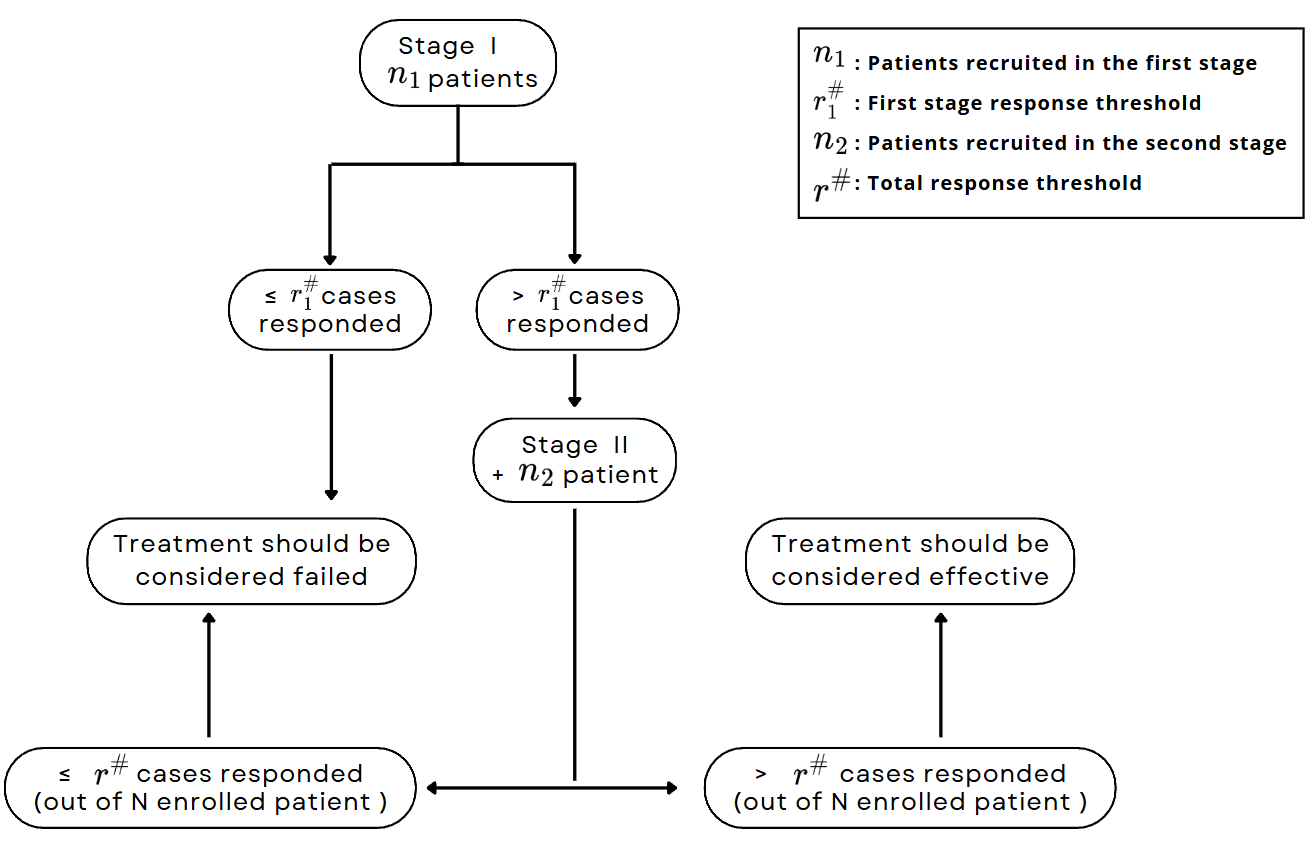
\includegraphics[width=1\linewidth, trim=0cm 0cm 0cm 0cm, clip]{simon optimal plot.png} % 调整 trim 参数裁剪图片边缘
    %\caption{PSO 演算法示意圖}
    \label{fig:pso}
\end{figure}
\end{frame}

\begin{frame}{Literature Review: Simon's Two-Stage Design}
\begin{columns}

    % 左側內容，減少寬度
    \column{0.58\textwidth}
    \begin{block}{Hypothesis Testing in Phase II Trials}
        \begin{itemize}
            \item \( H_0 : p \leq p_0 \)
            \item \( H_1 : p \geq p_1 \)
        \end{itemize}
        \vspace{0.3cm}
            \hspace{0.7cm}\( p_0 \): Unacceptable response level\\
            \hspace{0.7cm}\( p_1 \): Target response level
    \end{block}
    % 右側內容，增加寬度
    \column{0.42\textwidth}
    \begin{block}{Considerations}
        \begin{itemize}
        \small
            \item Constrained by \( \alpha \) and \( \beta \)
            \vspace{0.1cm}
            \item Reducing low-efficacy treatment exposure
        \end{itemize}
    \end{block}
\end{columns}
\vspace{0cm}
\end{frame}


\section{Expected Sample Size}

\begin{frame}{Probability of Early Termination at Each Stage}
\begin{block}{Binomial Distribution Formula}
\footnotesize
\[
b(x; n, p) = \binom{n}{x} p^x (1 - p)^{n - x}
\]
\end{block}
\vspace{-0.2cm}
\scriptsize
\begin{itemize} % 减少缩进
    \item \( n \): Total number of patients
    \item \( x \): Number of successes (responses)
    \item \( p \): Probability of success for each patient
\end{itemize}
\vspace{-0.2cm}

\begin{block}{Early Termination Probability (\(PET_1\))}
\footnotesize
\[
PET_1(p) = \sum_{x=0}^{r_1} b(x; n_1, p_0)
\]
\end{block}
\vspace{-0.2cm}
\scriptsize
\begin{itemize}
    \item \( n_1 \): Patients in the first stage
    \item \( r_1 \): Response threshold for the first stage
\end{itemize}
\end{frame}




\begin{frame}{Treatment Rejection and EN (2-Stage Design)}
\begin{block}{Rejection Probability (Second Stage)}
\[
\sum_{x_1 = r_1 + 1}^{\min[n_1, r_2]} b(x_1; n_1, p_0) B(r_2 - x_1; n_2, p_0)
\]
\end{block}

\begin{itemize}
\scriptsize
    \item \( n_1, n_2 \): Patients in stages 1 and 2
    \item \( r_1, r_2 \): Rejection thresholds for stages 1 and 2
    \item \( p \): Success probability
\end{itemize}

\begin{block}{Expected Sample Size (EN)}
\[
EN = n_1 + (1 - PET_1) n_2
\]
\end{block}
\begin{itemize}
\scriptsize
    \item \( PET_1 \): Probability of early termination (stage 1)
\end{itemize}
\end{frame}





\begin{frame}{Early Termination Probability (\( K \)-Stage Design)}
\begin{block}{Formula for \( PET_k(p) \)}
\footnotesize
\[
PET_k(p) = 
\underbrace{
\sum_{x_1 = L_1}^{U_1} \sum_{x_2 = L_2}^{U_2} \cdots \sum_{x_{k-1} = L_{k-1}}^{U_{k-1}}
}_{\text{\( k-1 \) Summations}}
\left[ \prod_{s=1}^{k-1} b(x_s; n_s, p_0) \right]
B\left( r_k = \sum_{s=1}^{k-1} x_s, n_k, p_0 \right)
\]
\end{block}

\scriptsize
\begin{itemize}
    \item \( b(x_s; n_s, p) \): Binomial probability at stage \( s \).
    \item \( L_j, U_j \): Lower and upper bounds of stage \( j \).
\end{itemize}

\begin{block}{Formula for Expected Sample Size (EN)}
\footnotesize
\[
EN = n_1 + (1 - PET_1) n_2 + \cdots + (1 - PET_{k-2}) n_{k-1} + (1 - PET_{k-1}) n_k
\]
\end{block}
% Explanation for EN as PSO Objective
\footnotesize
\begin{itemize}
\item (\( EN_{p_0} \)) is the primary  objective function of the PSO algorithm.
\end{itemize}
\end{frame}


\begin{frame}{Total Combination Possibilities}

% 表格部分
\begin{table}[t]
\centering
\resizebox{0.8\linewidth}{!}{% 限制表格宽度为 80%
\begin{tabular}{|c|c|c|c|c|c|}
\hline
$p_0$ & $p_1$ & Stage 1 & Stage 2 & \cellcolor{yellow!20}EN($p_0$) & PET$_1$($p_0$) \\
\hline
0.1 & 0.3 & 1/12 & 5/35 & \cellcolor{yellow!20}19.8 & 0.65 \\
\hline
\end{tabular}
}
\end{table}

% 调整表格和文字之间的间距
\vspace{0.1cm}

% 可能组合数量
\begin{itemize} % 增加条目间距
    \item \textbf{2-Stage Design:} \hspace*{1.5cm}\( 1,105,524 \) possibilities
    \item \textbf{3-Stage Design:} \hspace*{1.12cm}\( 213,672,935 \) possibilities
    \item \textbf{4-Stage Design:} \hspace*{0.56cm}\( 22,546,940,047 \) possibilities
    \item \textbf{5-Stage Design:} \( 1,530,973,869,444 \) possibilities
\end{itemize}

\vspace{0.5cm} % 调整说明文字与列表的间距

% 添加备注
\footnotesize
\textbf{Note:} Enumeration range: \\
\hspace*{1cm} Total sample size \( N = n_1 + \ldots + n_k \), where \( 30 \leq N \leq 70 \).

\end{frame}



\section{PSO Algorithm}
\begin{frame}
\frametitle{PSO(Particle Swarm Optimization)}
\begin{figure}
    \centering
    \hspace{0 cm} % 调整水平偏移
    \vspace{2 cm} % 调整垂直偏移
    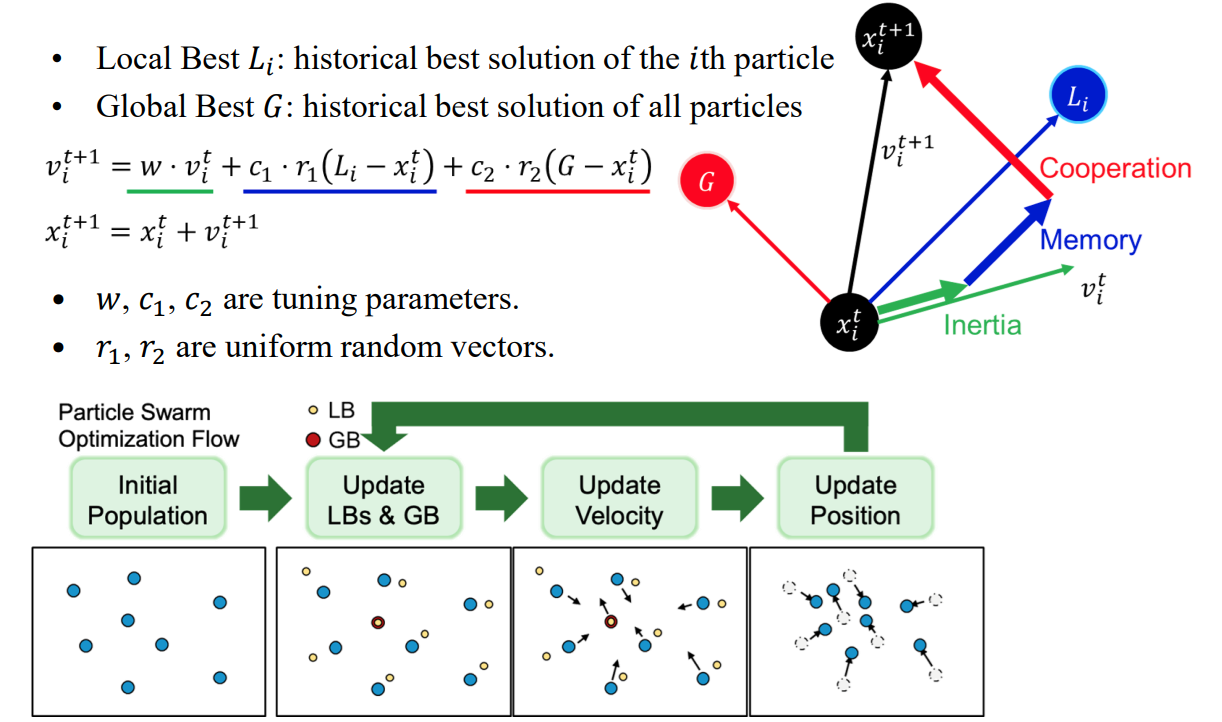
\includegraphics[width=1.05\linewidth]{PSO.png} % 確保圖片在與.tex文件相同的目錄
    %\caption{PSO 演算法示意圖}
    \label{fig:pso}
\end{figure}
\end{frame}



\section{Existing results}

\begin{frame}
\frametitle{3-stage Optimal Design}
% 三階段表格
\begin{center}
\resizebox{0.9\linewidth}{!}{% 控制表格缩放比例
\begin{tabular}{|c|c|c|c|c|>{\columncolor{yellow!30}}c|c|c|}
\hline
$p_0$ & $p_1$ & Stage 1 & Stage 2 & Stage 3 & EN($p_0$) & $PET_1$($p_0$) & $PET_2$($p_0$) \\
\hline
0.05 & 0.25 & 0/9 & 1/18 & 2/26 & 13.78 & 0.63 & 0.82 \\
0.10 & 0.30 & 0/10 & 2/19 & 4/26 & 17.79 & 0.35 & 0.72 \\
0.15 & 0.35 & 1/12 & 3/21 & 7/33 & 21.11 & 0.44 & 0.66 \\
0.20 & 0.40 & 1/10 & 6/26 & 11/43 & 23.86 & 0.38 & 0.77 \\
0.25 & 0.45 & 3/16 & 7/25 & 13/41 & 25.55 & 0.41 & 0.74 \\
0.30 & 0.50 & 3/13 & 9/28 & 17/46 & 26.75 & 0.42 & 0.7 \\
0.35 & 0.55 & 6/18 & 13/33 & 20/48 & 27.84 & 0.55 & 0.8 \\
0.40 & 0.60 & 6/17 & 12/28 & 21/44 & 27.59 & 0.45 & 0.72 \\
0.45 & 0.65 & 5/13 & 13/27 & 26/50 & 27.22 & 0.43 & 0.73 \\
0.50 & 0.70 & 4/10 & 13/25 & 27/47 & 26.08 & 0.38 & 0.69 \\
0.55 & 0.75 & 5/11 & 12/21 & 27/43 & 24.36 & 0.37 & 0.7 \\
0.60 & 0.80 & 6/11 & 14/22 & 29/43 & 22.30 & 0.47 & 0.74 \\
0.65 & 0.85 & 5/9 & 13/19 & 25/34 & 19.23 & 0.39 & 0.72 \\
0.70 & 0.90 & 5/8 & 11/15 & 22/28 & 15.45 & 0.45 & 0.72 \\
0.75 & 0.95 & 3/5 & 6/8 & 16/19 & 10.94 & 0.37 & 0.63 \\
\hline
\multicolumn{8}{|l|}{$p_1 -  p_0 =0.20$ and $\alpha = 0.10$ , $\beta = 0.10$} \\ % 这里指定8列，并放在一个完整的表格行中
\hline
\end{tabular}
}
\end{center}
\end{frame}


\begin{frame}
\frametitle{Chen 1997 vs. PSO Results}
\begin{center}
\textbf{Improved Combinations for 3-Stage Designs}
\end{center}
\resizebox{1\linewidth}{!}{%
\begin{tabular}{|c|c|c|c|c|c|c|c|c|}
\hline
$P_0$ & $P_1$ &  & Stage 1 & Stage 2 & Stage 3 & EN($p_0$) & PET1($p_0$) & PET2($p_0$) \\
\hline
\rowcolor{cyan!50} \multicolumn{9}{|c|}{$\alpha = 0.10$, $\beta = 0.10$} \\
\hline
\multirow{2}{*}{0.40} & \multirow{2}{*}{0.60} 
    & Chen & 7/18 & 9/26 & 22/46 & 29.81 & 0.56 & 0.58 \\ % Chen Result
\cline{3-9}
  &  & \cellcolor{yellow} PSO & \cellcolor{yellow} 6/17 & \cellcolor{yellow} 12/28 & \cellcolor{yellow} 21/44 & \cellcolor{yellow} 27.59 & \cellcolor{yellow} 0.45 & \cellcolor{yellow} 0.72 \\ % PSO Result
\hline
\multirow{2}{*}{0.50} & \multirow{2}{*}{0.70} 
    & Chen & 4/10 & 12/24 & 26/45 & 26.37 & 0.38 & 0.64 \\ % Chen Result
\cline{3-9}
  &  & \cellcolor{yellow} PSO & \cellcolor{yellow} 4/10 & \cellcolor{yellow} 13/25 & \cellcolor{yellow} 27/47 & \cellcolor{yellow} 26.08 & \cellcolor{yellow} 0.38 & \cellcolor{yellow} 0.69 \\ % PSO Result
\hline
\rowcolor{cyan!50} \multicolumn{9}{|c|}{$\alpha = 0.05$, $\beta = 0.20$} \\
\hline
\multirow{2}{*}{0.40} & \multirow{2}{*}{0.60} 
    & Chen & 3/9 & 10/23 & 23/46 & 21.74 & 0.48 & 0.76 \\ % Chen Result
\cline{3-9}
  &  & \cellcolor{yellow} PSO & \cellcolor{yellow} 3/9 & \cellcolor{yellow} 11/24 & \cellcolor{yellow} 25/51 & \cellcolor{yellow} 21.71 & \cellcolor{yellow} 0.48 & \cellcolor{yellow} 0.82 \\ % PSO Result
\hline
\end{tabular}
}
\end{frame}




\begin{frame}
\frametitle{4-stage Optimal Design}
% 四階段表格
\begin{center}
\resizebox{1\linewidth}{!}{% 将 0.9 调整为 0.95 或 0.85 以控制缩放比例
\begin{tabular}{|c|c|c|c|c|c|>{\columncolor{yellow!30}}c|c|c|c|}
\hline
$p_0$ & $p_1$ & Stage 1 & Stage 2 & Stage 3 & Stage 4 & EN($p_0$) & $PET_1$($p_0$) & $PET_2$($p_0$) & $PET_3$($p_0$) \\
\hline
0.05 & 0.25 & 0/9 & 0/17 & 1/18 & 2/26 & 13.78 & 0.63 & 0.63 & 0.82 \\
0.10 & 0.30 & 0/11 & 1/15 & 2/19 & 4/26 & 17.37 & 0.31 & 0.57 & 0.73 \\
0.15 & 0.35 & 0/9 & 2/16 & 4/26 & 7/33 & 20.55 & 0.23 & 0.58 & 0.72 \\
0.20 & 0.40 & 1/10 & 4/21 & 7/30 & 11/43 & 22.73 & 0.38 & 0.63 & 0.80 \\
0.25 & 0.45 & 1/10 & 4/18 & 8/28 & 14/45 & 24.42 & 0.24 & 0.54 & 0.78 \\
0.30 & 0.50 & 2/11 & 6/21 & 11/33 & 17/46 & 25.77 & 0.31 & 0.59 & 0.78 \\
0.35 & 0.55 & 4/14 & 10/27 & 15/38 & 20/48 & 26.55 & 0.42 & 0.70 & 0.82 \\
0.40 & 0.60 & 4/13 & 10/24 & 16/36 & 23/49 & 26.29 & 0.30 & 0.62 & 0.75 \\
0.45 & 0.65 & 3/10 & 9/20 & 16/33 & 25/48 & 25.81 & 0.27 & 0.61 & 0.77 \\
0.50 & 0.70 & 4/11 & 8/17 & 15/28 & 26/45 & 24.96 & 0.27 & 0.52 & 0.75 \\
0.55 & 0.75 & 5/11 & 10/18 & 19/32 & 28/45 & 23.20 & 0.37 & 0.63 & 0.76 \\
0.60 & 0.80 & 5/10 & 9/15 & 17/27 & 27/40 & 20.91 & 0.37 & 0.61 & 0.76 \\
0.65 & 0.85 & 5/9 & 13/19 & 20/28 & 24/33 & 18.32 & 0.39 & 0.72 & 0.75 \\
0.70 & 0.90 & 1/3 & 6/9 & 15/20 & 24/31 & 14.72 & 0.22 & 0.56 & 0.80 \\
0.75 & 0.95 & 3/5 & 6/8 & 11/14 & 16/19 & 10.23 & 0.37 & 0.63 & 0.77 \\
\hline
\multicolumn{10}{|l|}{$p_1 -  p_0 =0.20$ and $\alpha = 0.10$ , $\beta = 0.10$} \\ % 这里指定10列，并放在一个完整的表格行中
\hline
\end{tabular}
}
\end{center}
\end{frame}


\begin{frame}
\frametitle{EN($p_0$) Comparison between 3 \& 4-stage Designs}
\begin{center}
\tiny
\resizebox{0.8\linewidth}{!}{%
\begin{tabular}{|c|c|c|c|c|}
\hline
\multirow{2}{*}{$P_0$} & \multirow{2}{*}{$P_1$} & \multicolumn{2}{c|}{\cellcolor{cyan}EN($p_0$) (Optimal)} & \multirow{2}{*}{Variation}\\
\cline{3-4}
& & 3-stage & 4-stage & \\
\hline
0.05 & 0.25 & 13.78 & 13.78 & 0\\
0.10 & 0.30 & 17.79 & 17.37 & -0.42\\ % 更新后的4-stage数据
0.15 & 0.35 & 21.11 & 20.55 & -0.56\\
0.20 & 0.40 & 23.86 & 22.73 & -1.13\\
0.25 & 0.45 & 25.55 & 24.42 & -1.13\\
0.30 & 0.50 & 26.75 & 25.77 & -0.98\\
0.35 & 0.55 & 27.84 & 26.55 & -1.29\\
0.40 & 0.60 & 29.81 & 26.29 & -3.52\\
0.45 & 0.65 & 27.22 & 25.81 & -1.41\\
0.50 & 0.70 & 26.37 & 24.96 & -1.41\\
0.55 & 0.75 & 24.36 & 23.20 & -1.16\\
0.60 & 0.80 & 22.30 & 20.91 & -1.39\\ % 更新后的4-stage数据
0.65 & 0.85 & 19.23 & 18.32 & -0.91\\
0.70 & 0.90 & 15.45 & 14.72 & -0.73\\
0.75 & 0.95 & 10.94 & 10.23 & -0.71\\
\hline
\end{tabular}
}
\end{center}
\end{frame}



\section{Challenges, and Future Plans}

\begin{frame}
\frametitle{Challenges, and Future Plans}
\begin{itemize}
    \item \textbf{Challenges}:
    \begin{itemize}
        \item Stability issues, convergence speed, and sensitivity to parameters .
        \item Inconsistent results across multiple runs.
    \end{itemize}
    
    \item \textbf{Future Plans}:
    \begin{itemize}
    	\item Enhancing algorithm stability and convergence efficiency.
        \item Integrating \textbf{minimax design} into the algorithm.
        \item Adapting the Approach to Broader Clinical Trial Scenarios (e.g., Platform Trials).
    \end{itemize}
\end{itemize}
\end{frame}


\begin{frame}{References}
\small % 或者使用 \footnotesize 进一步缩小字体
\begin{itemize}
	\item Atkinson, A., Donev, A., Tobias, R. (2007). Optimum experimental designs, with SAS. OUP Oxford. (pp. 58-69, Chapter 6; pp. 119-147, Chapters 9-10).
	\item Chen, T. T. (1997). Optimal three-stage designs for phase II cancer clinical trials. Statistics in medicine, 16(23):2701–2711.
	\item Qiu, J., Chen, R.-B., Wang, W., and Wong, W. K. (2014). Using animal instincts to design efficient biomedical studies via particle swarm optimization. Swarm and evolutionary computation, 18:1–10.
    \item Simon, R. (1989). Optimal two-stage designs for phase ii clinical trials. Controlled clinical trials, 10(1):1–10.
    \item Yang, X.-S. (2010). Engineering optimization: an introduction with metaheuristic applications, pp. 29-35.
    
\end{itemize}
\end{frame}


\end{document}


